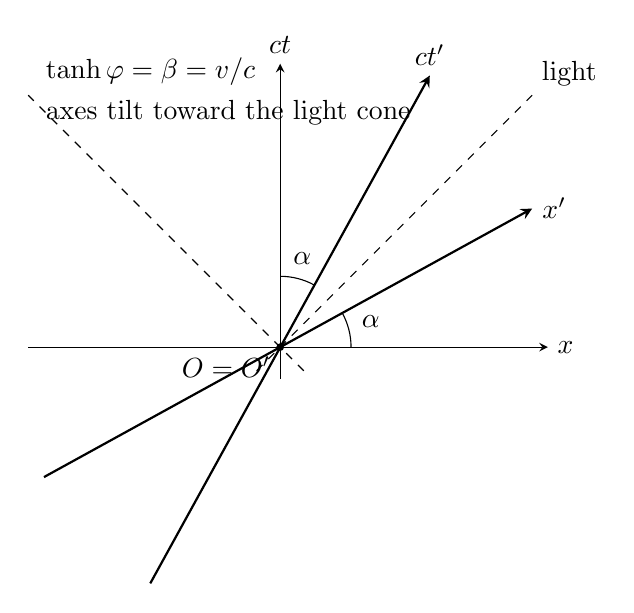
\begin{tikzpicture}[x=1cm,y=1cm,>=stealth]
    \def\v{0.55}
    \def\ang{28.8}

    \draw[->] (-3.2,0) -- (3.4,0) node[right] {\(x\)};
    \draw[->] (0,-0.4) -- (0,3.6) node[above] {\(ct\)};

    \draw[dashed] (-0.3,-0.3) -- (3.2,3.2) node[above right] {light};
    \draw[dashed] (0.3,-0.3) -- (-3.2,3.2);

    % x' axis: ct' = 0 -> ct = beta x
    \draw[thick,->] (-3.0,-1.65) -- (3.2,1.76) node[right] {\(x'\)};
    % ct' axis: x' = 0 -> x = beta ct
    \draw[thick,->] (-1.65,-3.0) -- (1.9,3.45) node[above] {\(ct'\)};

    \fill (0,0) circle (1.4pt) node[below left] {\(O=O'\)};

    \draw (0.9,0) arc (0:28.8:0.9);
    \node at (1.15,0.32) {\(\alpha\)};
    \draw (0,0.9) arc (90:61.2:0.9);
    \node at (0.28,1.13) {\(\alpha\)};

    \node[align=left,anchor=west] at (-3.1,3.25)
    {\(\tanh\varphi=\beta=v/c\)\\[1mm]
     axes tilt toward the light cone};
\end{tikzpicture}
